% Created by tikzDevice version 0.12.6 on 2025-04-07 13:16:19
% !TEX encoding = UTF-8 Unicode
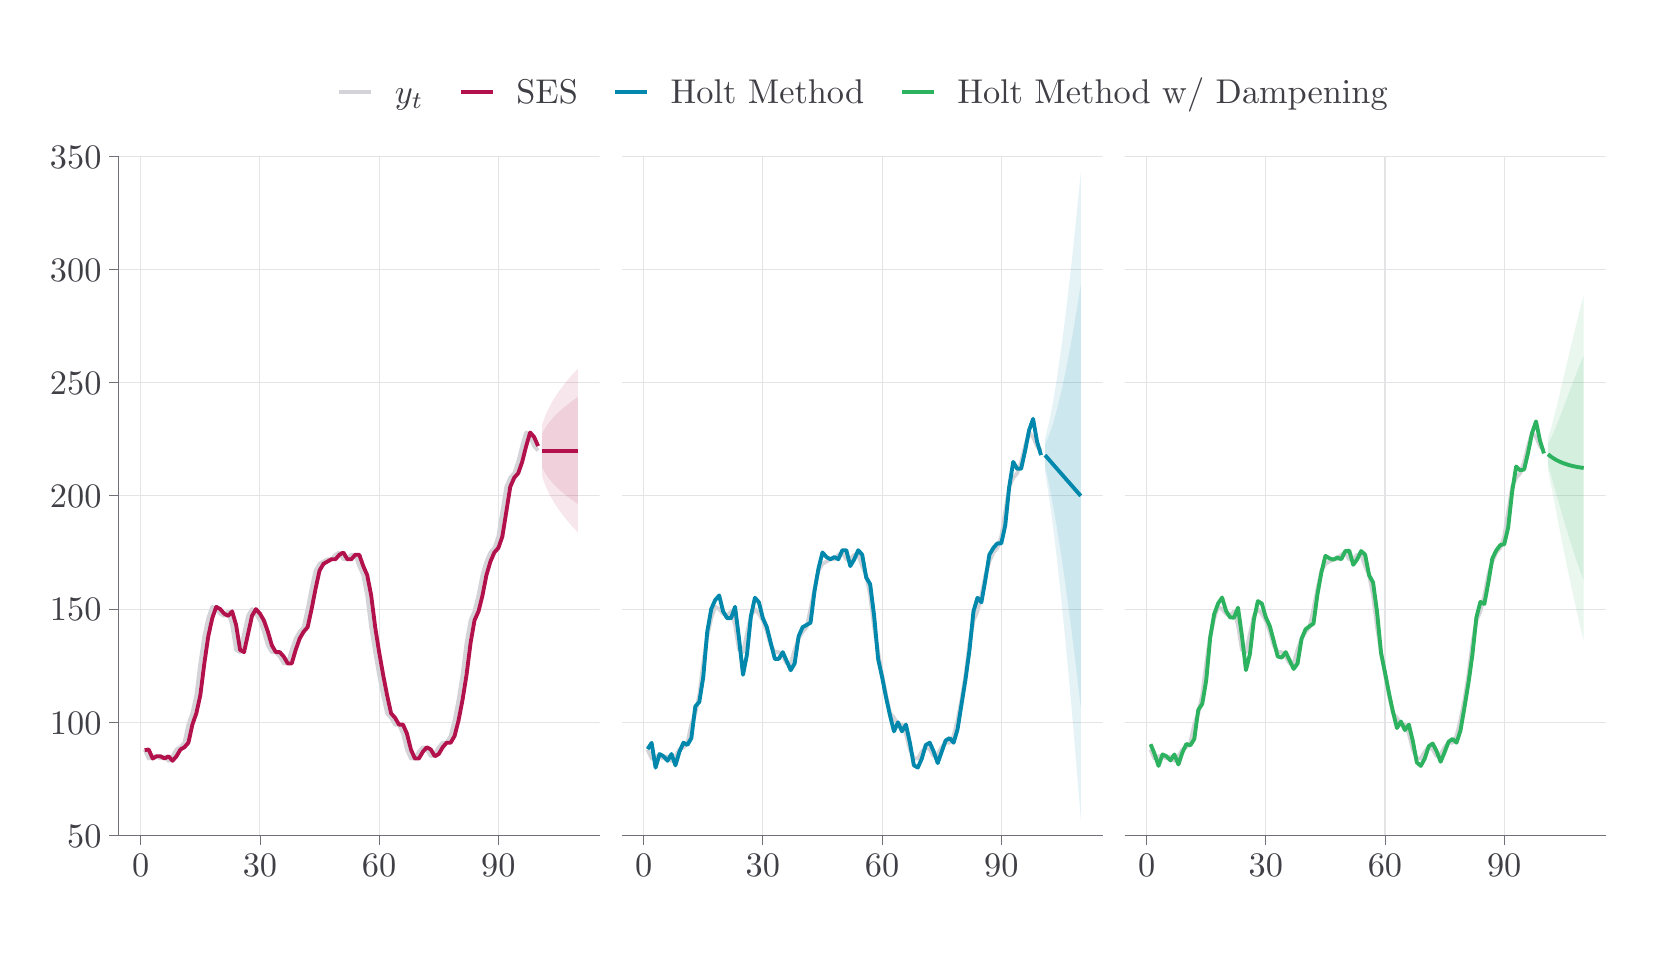
\begin{tikzpicture}[x=1pt,y=1pt]
\definecolor{fillColor}{RGB}{255,255,255}
\path[use as bounding box,fill=fillColor] (0,0) rectangle (578.16,325.21);
\begin{scope}
\path[clip] (  0.00,  0.00) rectangle (578.16,325.21);
\definecolor{drawColor}{RGB}{255,255,255}

\path[draw=drawColor,line width= 0.6pt,line join=round,line cap=round,fill=fillColor] ( -0.00,  0.00) rectangle (578.16,325.21);
\end{scope}
\begin{scope}
\path[clip] (  4.00,  8.00) rectangle (210.69,317.21);
\definecolor{drawColor}{RGB}{255,255,255}
\definecolor{fillColor}{RGB}{255,255,255}

\path[draw=drawColor,line width= 0.7pt,line join=round,line cap=round,fill=fillColor] (  4.00,  8.00) rectangle (210.69,317.21);
\end{scope}
\begin{scope}
\path[clip] (210.69,  8.00) rectangle (392.43,317.21);
\definecolor{drawColor}{RGB}{255,255,255}
\definecolor{fillColor}{RGB}{255,255,255}

\path[draw=drawColor,line width= 0.7pt,line join=round,line cap=round,fill=fillColor] (210.69,  8.00) rectangle (392.43,317.21);
\end{scope}
\begin{scope}
\path[clip] (392.43,  8.00) rectangle (574.16,317.21);
\definecolor{drawColor}{RGB}{255,255,255}
\definecolor{fillColor}{RGB}{255,255,255}

\path[draw=drawColor,line width= 0.7pt,line join=round,line cap=round,fill=fillColor] (392.43,  8.00) rectangle (574.16,317.21);
\end{scope}
\begin{scope}
\path[clip] ( 32.96, 33.29) rectangle (206.69,278.76);
\definecolor{drawColor}{RGB}{255,255,255}
\definecolor{fillColor}{RGB}{255,255,255}

\path[draw=drawColor,line width= 0.7pt,line join=round,line cap=round,fill=fillColor] ( 32.96, 33.29) rectangle (206.69,278.76);
\definecolor{drawColor}{RGB}{228,228,231}

\path[draw=drawColor,line width= 0.4pt,line join=round] ( 32.96, 33.29) --
	(206.69, 33.29);

\path[draw=drawColor,line width= 0.4pt,line join=round] ( 32.96, 74.20) --
	(206.69, 74.20);

\path[draw=drawColor,line width= 0.4pt,line join=round] ( 32.96,115.11) --
	(206.69,115.11);

\path[draw=drawColor,line width= 0.4pt,line join=round] ( 32.96,156.02) --
	(206.69,156.02);

\path[draw=drawColor,line width= 0.4pt,line join=round] ( 32.96,196.94) --
	(206.69,196.94);

\path[draw=drawColor,line width= 0.4pt,line join=round] ( 32.96,237.85) --
	(206.69,237.85);

\path[draw=drawColor,line width= 0.4pt,line join=round] ( 32.96,278.76) --
	(206.69,278.76);

\path[draw=drawColor,line width= 0.4pt,line join=round] ( 40.85, 33.29) --
	( 40.85,278.76);

\path[draw=drawColor,line width= 0.4pt,line join=round] ( 83.93, 33.29) --
	( 83.93,278.76);

\path[draw=drawColor,line width= 0.4pt,line join=round] (127.00, 33.29) --
	(127.00,278.76);

\path[draw=drawColor,line width= 0.4pt,line join=round] (170.08, 33.29) --
	(170.08,278.76);
\definecolor{drawColor}{RGB}{212,212,216}

\path[draw=drawColor,line width= 1.4pt,line join=round] ( 42.29, 64.38) --
	( 43.72, 61.11) --
	( 45.16, 61.92) --
	( 46.60, 61.92) --
	( 48.03, 61.11) --
	( 49.47, 61.92) --
	( 50.90, 60.29) --
	( 52.34, 61.92) --
	( 53.77, 64.38) --
	( 55.21, 65.20) --
	( 56.65, 66.83) --
	( 58.08, 73.38) --
	( 59.52, 77.47) --
	( 60.95, 84.02) --
	( 62.39, 95.47) --
	( 63.83,105.29) --
	( 65.26,111.84) --
	( 66.70,115.93) --
	( 68.13,115.11) --
	( 69.57,113.47) --
	( 71.00,112.66) --
	( 72.44,114.29) --
	( 73.88,109.38) --
	( 75.31,100.38) --
	( 76.75, 99.56) --
	( 78.18,106.11) --
	( 79.62,112.66) --
	( 81.06,115.11) --
	( 82.49,113.47) --
	( 83.93,111.02) --
	( 85.36,106.93) --
	( 86.80,102.02) --
	( 88.23, 99.56) --
	( 89.67, 99.56) --
	( 91.11, 97.93) --
	( 92.54, 95.47) --
	( 93.98, 95.47) --
	( 95.41,100.38) --
	( 96.85,104.47) --
	( 98.29,106.93) --
	( 99.72,108.56) --
	(101.16,115.11) --
	(102.59,122.48) --
	(104.03,129.02) --
	(105.46,131.48) --
	(106.90,132.29) --
	(108.34,133.11) --
	(109.77,133.11) --
	(111.21,134.75) --
	(112.64,135.57) --
	(114.08,133.11) --
	(115.52,133.11) --
	(116.95,134.75) --
	(118.39,134.75) --
	(119.82,130.66) --
	(121.26,127.38) --
	(122.69,120.02) --
	(124.13,108.56) --
	(125.57, 99.56) --
	(127.00, 91.38) --
	(128.44, 84.02) --
	(129.87, 77.47) --
	(131.31, 75.83) --
	(132.75, 73.38) --
	(134.18, 73.38) --
	(135.62, 70.11) --
	(137.05, 64.38) --
	(138.49, 61.11) --
	(139.92, 61.11) --
	(141.36, 63.56) --
	(142.80, 65.20) --
	(144.23, 64.38) --
	(145.67, 61.92) --
	(147.10, 62.74) --
	(148.54, 65.20) --
	(149.98, 66.83) --
	(151.41, 66.83) --
	(152.85, 69.29) --
	(154.28, 75.02) --
	(155.72, 82.38) --
	(157.15, 91.38) --
	(158.59,102.84) --
	(160.03,111.02) --
	(161.46,114.29) --
	(162.90,120.02) --
	(164.33,127.38) --
	(165.77,132.29) --
	(167.21,135.57) --
	(168.64,137.20) --
	(170.08,141.29) --
	(171.51,150.30) --
	(172.95,159.30) --
	(174.38,162.57) --
	(175.82,164.21) --
	(177.26,168.30) --
	(178.69,174.02) --
	(180.13,178.93) --
	(181.56,177.30) --
	(183.00,174.02) --
	(184.44,172.39);
\definecolor{drawColor}{RGB}{179,17,75}

\path[draw=drawColor,line width= 1.4pt,line join=round] ( 42.29, 64.14) --
	( 43.72, 64.38) --
	( 45.16, 61.11) --
	( 46.60, 61.92) --
	( 48.03, 61.92) --
	( 49.47, 61.11) --
	( 50.90, 61.92) --
	( 52.34, 60.29) --
	( 53.77, 61.92) --
	( 55.21, 64.38) --
	( 56.65, 65.20) --
	( 58.08, 66.83) --
	( 59.52, 73.38) --
	( 60.95, 77.47) --
	( 62.39, 84.02) --
	( 63.83, 95.47) --
	( 65.26,105.29) --
	( 66.70,111.84) --
	( 68.13,115.93) --
	( 69.57,115.11) --
	( 71.00,113.47) --
	( 72.44,112.66) --
	( 73.88,114.29) --
	( 75.31,109.38) --
	( 76.75,100.38) --
	( 78.18, 99.56) --
	( 79.62,106.11) --
	( 81.06,112.66) --
	( 82.49,115.11) --
	( 83.93,113.47) --
	( 85.36,111.02) --
	( 86.80,106.93) --
	( 88.23,102.02) --
	( 89.67, 99.56) --
	( 91.11, 99.56) --
	( 92.54, 97.93) --
	( 93.98, 95.47) --
	( 95.41, 95.47) --
	( 96.85,100.38) --
	( 98.29,104.47) --
	( 99.72,106.93) --
	(101.16,108.56) --
	(102.59,115.11) --
	(104.03,122.47) --
	(105.46,129.02) --
	(106.90,131.48) --
	(108.34,132.29) --
	(109.77,133.11) --
	(111.21,133.11) --
	(112.64,134.75) --
	(114.08,135.57) --
	(115.52,133.11) --
	(116.95,133.11) --
	(118.39,134.75) --
	(119.82,134.75) --
	(121.26,130.66) --
	(122.69,127.39) --
	(124.13,120.02) --
	(125.57,108.57) --
	(127.00, 99.57) --
	(128.44, 91.38) --
	(129.87, 84.02) --
	(131.31, 77.47) --
	(132.75, 75.84) --
	(134.18, 73.38) --
	(135.62, 73.38) --
	(137.05, 70.11) --
	(138.49, 64.38) --
	(139.92, 61.11) --
	(141.36, 61.11) --
	(142.80, 63.56) --
	(144.23, 65.20) --
	(145.67, 64.38) --
	(147.10, 61.92) --
	(148.54, 62.74) --
	(149.98, 65.20) --
	(151.41, 66.83) --
	(152.85, 66.83) --
	(154.28, 69.29) --
	(155.72, 75.02) --
	(157.15, 82.38) --
	(158.59, 91.38) --
	(160.03,102.84) --
	(161.46,111.02) --
	(162.90,114.29) --
	(164.33,120.02) --
	(165.77,127.38) --
	(167.21,132.29) --
	(168.64,135.57) --
	(170.08,137.20) --
	(171.51,141.29) --
	(172.95,150.29) --
	(174.38,159.30) --
	(175.82,162.57) --
	(177.26,164.21) --
	(178.69,168.30) --
	(180.13,174.02) --
	(181.56,178.93) --
	(183.00,177.30) --
	(184.44,174.03);

\path[draw=drawColor,line width= 1.4pt,line join=round] (185.87,172.39) --
	(187.31,172.39) --
	(188.74,172.39) --
	(190.18,172.39) --
	(191.61,172.39) --
	(193.05,172.39) --
	(194.49,172.39) --
	(195.92,172.39) --
	(197.36,172.39) --
	(198.79,172.39);
\definecolor{fillColor}{RGB}{179,17,75}

\path[fill=fillColor,fill opacity=0.10] (185.87,178.50) --
	(187.31,181.03) --
	(188.74,182.98) --
	(190.18,184.61) --
	(191.61,186.06) --
	(193.05,187.36) --
	(194.49,188.56) --
	(195.92,189.68) --
	(197.36,190.73) --
	(198.79,191.72) --
	(198.79,153.06) --
	(197.36,154.05) --
	(195.92,155.10) --
	(194.49,156.22) --
	(193.05,157.42) --
	(191.61,158.72) --
	(190.18,160.16) --
	(188.74,161.80) --
	(187.31,163.74) --
	(185.87,166.28) --
	cycle;

\path[] (185.87,178.50) --
	(187.31,181.03) --
	(188.74,182.98) --
	(190.18,184.61) --
	(191.61,186.06) --
	(193.05,187.36) --
	(194.49,188.56) --
	(195.92,189.68) --
	(197.36,190.73) --
	(198.79,191.72);

\path[] (198.79,153.06) --
	(197.36,154.05) --
	(195.92,155.10) --
	(194.49,156.22) --
	(193.05,157.42) --
	(191.61,158.72) --
	(190.18,160.16) --
	(188.74,161.80) --
	(187.31,163.74) --
	(185.87,166.28);

\path[fill=fillColor,fill opacity=0.10] (185.87,181.74) --
	(187.31,185.61) --
	(188.74,188.58) --
	(190.18,191.09) --
	(191.61,193.29) --
	(193.05,195.29) --
	(194.49,197.12) --
	(195.92,198.83) --
	(197.36,200.43) --
	(198.79,201.95) --
	(198.79,142.83) --
	(197.36,144.34) --
	(195.92,145.95) --
	(194.49,147.65) --
	(193.05,149.49) --
	(191.61,151.48) --
	(190.18,153.69) --
	(188.74,156.20) --
	(187.31,159.17) --
	(185.87,163.04) --
	cycle;

\path[] (185.87,181.74) --
	(187.31,185.61) --
	(188.74,188.58) --
	(190.18,191.09) --
	(191.61,193.29) --
	(193.05,195.29) --
	(194.49,197.12) --
	(195.92,198.83) --
	(197.36,200.43) --
	(198.79,201.95);

\path[] (198.79,142.83) --
	(197.36,144.34) --
	(195.92,145.95) --
	(194.49,147.65) --
	(193.05,149.49) --
	(191.61,151.48) --
	(190.18,153.69) --
	(188.74,156.20) --
	(187.31,159.17) --
	(185.87,163.04);
\end{scope}
\begin{scope}
\path[clip] (  0.00,  0.00) rectangle (578.16,325.21);
\definecolor{drawColor}{RGB}{113,113,122}

\path[draw=drawColor,line width= 0.3pt,line join=round] ( 32.96, 33.29) --
	( 32.96,278.76);
\end{scope}
\begin{scope}
\path[clip] (  0.00,  0.00) rectangle (578.16,325.21);
\definecolor{drawColor}{RGB}{63,63,70}

\node[text=drawColor,anchor=base east,inner sep=0pt, outer sep=0pt, scale=  1.24] at ( 26.66, 29.00) {50};

\node[text=drawColor,anchor=base east,inner sep=0pt, outer sep=0pt, scale=  1.24] at ( 26.66, 69.91) {100};

\node[text=drawColor,anchor=base east,inner sep=0pt, outer sep=0pt, scale=  1.24] at ( 26.66,110.83) {150};

\node[text=drawColor,anchor=base east,inner sep=0pt, outer sep=0pt, scale=  1.24] at ( 26.66,151.74) {200};

\node[text=drawColor,anchor=base east,inner sep=0pt, outer sep=0pt, scale=  1.24] at ( 26.66,192.65) {250};

\node[text=drawColor,anchor=base east,inner sep=0pt, outer sep=0pt, scale=  1.24] at ( 26.66,233.56) {300};

\node[text=drawColor,anchor=base east,inner sep=0pt, outer sep=0pt, scale=  1.24] at ( 26.66,274.48) {350};
\end{scope}
\begin{scope}
\path[clip] (  0.00,  0.00) rectangle (578.16,325.21);
\definecolor{drawColor}{RGB}{113,113,122}

\path[draw=drawColor,line width= 0.3pt,line join=round] ( 29.46, 33.29) --
	( 32.96, 33.29);

\path[draw=drawColor,line width= 0.3pt,line join=round] ( 29.46, 74.20) --
	( 32.96, 74.20);

\path[draw=drawColor,line width= 0.3pt,line join=round] ( 29.46,115.11) --
	( 32.96,115.11);

\path[draw=drawColor,line width= 0.3pt,line join=round] ( 29.46,156.02) --
	( 32.96,156.02);

\path[draw=drawColor,line width= 0.3pt,line join=round] ( 29.46,196.94) --
	( 32.96,196.94);

\path[draw=drawColor,line width= 0.3pt,line join=round] ( 29.46,237.85) --
	( 32.96,237.85);

\path[draw=drawColor,line width= 0.3pt,line join=round] ( 29.46,278.76) --
	( 32.96,278.76);
\end{scope}
\begin{scope}
\path[clip] (  0.00,  0.00) rectangle (578.16,325.21);
\definecolor{drawColor}{RGB}{113,113,122}

\path[draw=drawColor,line width= 0.3pt,line join=round] ( 32.96, 33.29) --
	(206.69, 33.29);
\end{scope}
\begin{scope}
\path[clip] (  0.00,  0.00) rectangle (578.16,325.21);
\definecolor{drawColor}{RGB}{113,113,122}

\path[draw=drawColor,line width= 0.3pt,line join=round] ( 40.85, 29.79) --
	( 40.85, 33.29);

\path[draw=drawColor,line width= 0.3pt,line join=round] ( 83.93, 29.79) --
	( 83.93, 33.29);

\path[draw=drawColor,line width= 0.3pt,line join=round] (127.00, 29.79) --
	(127.00, 33.29);

\path[draw=drawColor,line width= 0.3pt,line join=round] (170.08, 29.79) --
	(170.08, 33.29);
\end{scope}
\begin{scope}
\path[clip] (  0.00,  0.00) rectangle (578.16,325.21);
\definecolor{drawColor}{RGB}{63,63,70}

\node[text=drawColor,anchor=base,inner sep=0pt, outer sep=0pt, scale=  1.24] at ( 40.85, 18.42) {0};

\node[text=drawColor,anchor=base,inner sep=0pt, outer sep=0pt, scale=  1.24] at ( 83.93, 18.42) {30};

\node[text=drawColor,anchor=base,inner sep=0pt, outer sep=0pt, scale=  1.24] at (127.00, 18.42) {60};

\node[text=drawColor,anchor=base,inner sep=0pt, outer sep=0pt, scale=  1.24] at (170.08, 18.42) {90};
\end{scope}
\begin{scope}
\path[clip] (214.69, 33.29) rectangle (388.43,278.76);
\definecolor{drawColor}{RGB}{255,255,255}
\definecolor{fillColor}{RGB}{255,255,255}

\path[draw=drawColor,line width= 0.7pt,line join=round,line cap=round,fill=fillColor] (214.69, 33.29) rectangle (388.43,278.76);
\definecolor{drawColor}{RGB}{228,228,231}

\path[draw=drawColor,line width= 0.4pt,line join=round] (214.69, 33.29) --
	(388.43, 33.29);

\path[draw=drawColor,line width= 0.4pt,line join=round] (214.69, 74.20) --
	(388.43, 74.20);

\path[draw=drawColor,line width= 0.4pt,line join=round] (214.69,115.11) --
	(388.43,115.11);

\path[draw=drawColor,line width= 0.4pt,line join=round] (214.69,156.02) --
	(388.43,156.02);

\path[draw=drawColor,line width= 0.4pt,line join=round] (214.69,196.94) --
	(388.43,196.94);

\path[draw=drawColor,line width= 0.4pt,line join=round] (214.69,237.85) --
	(388.43,237.85);

\path[draw=drawColor,line width= 0.4pt,line join=round] (214.69,278.76) --
	(388.43,278.76);

\path[draw=drawColor,line width= 0.4pt,line join=round] (222.59, 33.29) --
	(222.59,278.76);

\path[draw=drawColor,line width= 0.4pt,line join=round] (265.66, 33.29) --
	(265.66,278.76);

\path[draw=drawColor,line width= 0.4pt,line join=round] (308.74, 33.29) --
	(308.74,278.76);

\path[draw=drawColor,line width= 0.4pt,line join=round] (351.81, 33.29) --
	(351.81,278.76);
\definecolor{drawColor}{RGB}{212,212,216}

\path[draw=drawColor,line width= 1.4pt,line join=round] (224.02, 64.38) --
	(225.46, 61.11) --
	(226.89, 61.92) --
	(228.33, 61.92) --
	(229.77, 61.11) --
	(231.20, 61.92) --
	(232.64, 60.29) --
	(234.07, 61.92) --
	(235.51, 64.38) --
	(236.95, 65.20) --
	(238.38, 66.83) --
	(239.82, 73.38) --
	(241.25, 77.47) --
	(242.69, 84.02) --
	(244.12, 95.47) --
	(245.56,105.29) --
	(247.00,111.84) --
	(248.43,115.93) --
	(249.87,115.11) --
	(251.30,113.47) --
	(252.74,112.66) --
	(254.18,114.29) --
	(255.61,109.38) --
	(257.05,100.38) --
	(258.48, 99.56) --
	(259.92,106.11) --
	(261.35,112.66) --
	(262.79,115.11) --
	(264.23,113.47) --
	(265.66,111.02) --
	(267.10,106.93) --
	(268.53,102.02) --
	(269.97, 99.56) --
	(271.41, 99.56) --
	(272.84, 97.93) --
	(274.28, 95.47) --
	(275.71, 95.47) --
	(277.15,100.38) --
	(278.58,104.47) --
	(280.02,106.93) --
	(281.46,108.56) --
	(282.89,115.11) --
	(284.33,122.48) --
	(285.76,129.02) --
	(287.20,131.48) --
	(288.64,132.29) --
	(290.07,133.11) --
	(291.51,133.11) --
	(292.94,134.75) --
	(294.38,135.57) --
	(295.81,133.11) --
	(297.25,133.11) --
	(298.69,134.75) --
	(300.12,134.75) --
	(301.56,130.66) --
	(302.99,127.38) --
	(304.43,120.02) --
	(305.87,108.56) --
	(307.30, 99.56) --
	(308.74, 91.38) --
	(310.17, 84.02) --
	(311.61, 77.47) --
	(313.04, 75.83) --
	(314.48, 73.38) --
	(315.92, 73.38) --
	(317.35, 70.11) --
	(318.79, 64.38) --
	(320.22, 61.11) --
	(321.66, 61.11) --
	(323.10, 63.56) --
	(324.53, 65.20) --
	(325.97, 64.38) --
	(327.40, 61.92) --
	(328.84, 62.74) --
	(330.27, 65.20) --
	(331.71, 66.83) --
	(333.15, 66.83) --
	(334.58, 69.29) --
	(336.02, 75.02) --
	(337.45, 82.38) --
	(338.89, 91.38) --
	(340.33,102.84) --
	(341.76,111.02) --
	(343.20,114.29) --
	(344.63,120.02) --
	(346.07,127.38) --
	(347.50,132.29) --
	(348.94,135.57) --
	(350.38,137.20) --
	(351.81,141.29) --
	(353.25,150.30) --
	(354.68,159.30) --
	(356.12,162.57) --
	(357.55,164.21) --
	(358.99,168.30) --
	(360.43,174.02) --
	(361.86,178.93) --
	(363.30,177.30) --
	(364.73,174.02) --
	(366.17,172.39);
\definecolor{drawColor}{RGB}{1,136,172}

\path[draw=drawColor,line width= 1.4pt,line join=round] (224.02, 64.53) --
	(225.46, 66.77) --
	(226.89, 57.83) --
	(228.33, 62.74) --
	(229.77, 61.93) --
	(231.20, 60.29) --
	(232.64, 62.74) --
	(234.07, 58.65) --
	(235.51, 63.56) --
	(236.95, 66.83) --
	(238.38, 66.02) --
	(239.82, 68.47) --
	(241.25, 79.93) --
	(242.69, 81.56) --
	(244.12, 90.56) --
	(245.56,106.93) --
	(247.00,115.11) --
	(248.43,118.38) --
	(249.87,120.02) --
	(251.30,114.29) --
	(252.74,111.84) --
	(254.18,111.84) --
	(255.61,115.93) --
	(257.05,104.48) --
	(258.48, 91.38) --
	(259.92, 98.74) --
	(261.35,112.66) --
	(262.79,119.20) --
	(264.23,117.57) --
	(265.66,111.84) --
	(267.10,108.56) --
	(268.53,102.84) --
	(269.97, 97.11) --
	(271.41, 97.11) --
	(272.84, 99.56) --
	(274.28, 96.29) --
	(275.71, 93.02) --
	(277.15, 95.47) --
	(278.58,105.29) --
	(280.02,108.57) --
	(281.46,109.38) --
	(282.89,110.20) --
	(284.33,121.66) --
	(285.76,129.84) --
	(287.20,135.57) --
	(288.64,133.93) --
	(290.07,133.11) --
	(291.51,133.93) --
	(292.94,133.11) --
	(294.38,136.39) --
	(295.81,136.39) --
	(297.25,130.66) --
	(298.69,133.11) --
	(300.12,136.39) --
	(301.56,134.75) --
	(302.99,126.57) --
	(304.43,124.11) --
	(305.87,112.66) --
	(307.30, 97.11) --
	(308.74, 90.56) --
	(310.17, 83.20) --
	(311.61, 76.65) --
	(313.04, 70.93) --
	(314.48, 74.20) --
	(315.92, 70.93) --
	(317.35, 73.38) --
	(318.79, 66.84) --
	(320.22, 58.65) --
	(321.66, 57.83) --
	(323.10, 61.11) --
	(324.53, 66.02) --
	(325.97, 66.83) --
	(327.40, 63.56) --
	(328.84, 59.47) --
	(330.27, 63.56) --
	(331.71, 67.65) --
	(333.15, 68.47) --
	(334.58, 66.83) --
	(336.02, 71.74) --
	(337.45, 80.74) --
	(338.89, 89.75) --
	(340.33,100.38) --
	(341.76,114.29) --
	(343.20,119.20) --
	(344.63,117.57) --
	(346.07,125.75) --
	(347.50,134.75) --
	(348.94,137.20) --
	(350.38,138.84) --
	(351.81,138.84) --
	(353.25,145.39) --
	(354.68,159.30) --
	(356.12,168.30) --
	(357.55,165.84) --
	(358.99,165.84) --
	(360.43,172.39) --
	(361.86,179.75) --
	(363.30,183.84) --
	(364.73,175.66) --
	(366.17,170.75);

\path[draw=drawColor,line width= 1.4pt,line join=round] (367.61,170.75) --
	(369.04,169.11) --
	(370.48,167.48) --
	(371.91,165.84) --
	(373.35,164.20) --
	(374.78,162.57) --
	(376.22,160.93) --
	(377.66,159.29) --
	(379.09,157.66) --
	(380.53,156.02);
\definecolor{fillColor}{RGB}{1,136,172}

\path[fill=fillColor,fill opacity=0.10] (367.61,174.64) --
	(369.04,177.82) --
	(370.48,182.04) --
	(371.91,187.15) --
	(373.35,193.06) --
	(374.78,199.69) --
	(376.22,206.97) --
	(377.66,214.87) --
	(379.09,223.35) --
	(380.53,232.37) --
	(380.53, 79.67) --
	(379.09, 91.97) --
	(377.66,103.72) --
	(376.22,114.89) --
	(374.78,125.45) --
	(373.35,135.35) --
	(371.91,144.53) --
	(370.48,152.92) --
	(369.04,160.41) --
	(367.61,166.86) --
	cycle;

\path[] (367.61,174.64) --
	(369.04,177.82) --
	(370.48,182.04) --
	(371.91,187.15) --
	(373.35,193.06) --
	(374.78,199.69) --
	(376.22,206.97) --
	(377.66,214.87) --
	(379.09,223.35) --
	(380.53,232.37);

\path[] (380.53, 79.67) --
	(379.09, 91.97) --
	(377.66,103.72) --
	(376.22,114.89) --
	(374.78,125.45) --
	(373.35,135.35) --
	(371.91,144.53) --
	(370.48,152.92) --
	(369.04,160.41) --
	(367.61,166.86);

\path[fill=fillColor,fill opacity=0.10] (367.61,176.70) --
	(369.04,182.42) --
	(370.48,189.74) --
	(371.91,198.44) --
	(373.35,208.34) --
	(374.78,219.33) --
	(376.22,231.34) --
	(377.66,244.29) --
	(379.09,258.12) --
	(380.53,272.78) --
	(380.53, 39.26) --
	(379.09, 57.20) --
	(377.66, 74.30) --
	(376.22, 90.52) --
	(374.78,105.80) --
	(373.35,120.07) --
	(371.91,133.25) --
	(370.48,145.21) --
	(369.04,155.81) --
	(367.61,164.80) --
	cycle;

\path[] (367.61,176.70) --
	(369.04,182.42) --
	(370.48,189.74) --
	(371.91,198.44) --
	(373.35,208.34) --
	(374.78,219.33) --
	(376.22,231.34) --
	(377.66,244.29) --
	(379.09,258.12) --
	(380.53,272.78);

\path[] (380.53, 39.26) --
	(379.09, 57.20) --
	(377.66, 74.30) --
	(376.22, 90.52) --
	(374.78,105.80) --
	(373.35,120.07) --
	(371.91,133.25) --
	(370.48,145.21) --
	(369.04,155.81) --
	(367.61,164.80);
\end{scope}
\begin{scope}
\path[clip] (  0.00,  0.00) rectangle (578.16,325.21);
\definecolor{drawColor}{RGB}{113,113,122}

\path[draw=drawColor,line width= 0.3pt,line join=round] (214.69, 33.29) --
	(388.43, 33.29);
\end{scope}
\begin{scope}
\path[clip] (  0.00,  0.00) rectangle (578.16,325.21);
\definecolor{drawColor}{RGB}{113,113,122}

\path[draw=drawColor,line width= 0.3pt,line join=round] (222.59, 29.79) --
	(222.59, 33.29);

\path[draw=drawColor,line width= 0.3pt,line join=round] (265.66, 29.79) --
	(265.66, 33.29);

\path[draw=drawColor,line width= 0.3pt,line join=round] (308.74, 29.79) --
	(308.74, 33.29);

\path[draw=drawColor,line width= 0.3pt,line join=round] (351.81, 29.79) --
	(351.81, 33.29);
\end{scope}
\begin{scope}
\path[clip] (  0.00,  0.00) rectangle (578.16,325.21);
\definecolor{drawColor}{RGB}{63,63,70}

\node[text=drawColor,anchor=base,inner sep=0pt, outer sep=0pt, scale=  1.24] at (222.59, 18.42) {0};

\node[text=drawColor,anchor=base,inner sep=0pt, outer sep=0pt, scale=  1.24] at (265.66, 18.42) {30};

\node[text=drawColor,anchor=base,inner sep=0pt, outer sep=0pt, scale=  1.24] at (308.74, 18.42) {60};

\node[text=drawColor,anchor=base,inner sep=0pt, outer sep=0pt, scale=  1.24] at (351.81, 18.42) {90};
\end{scope}
\begin{scope}
\path[clip] (396.43, 33.29) rectangle (570.16,278.76);
\definecolor{drawColor}{RGB}{255,255,255}
\definecolor{fillColor}{RGB}{255,255,255}

\path[draw=drawColor,line width= 0.7pt,line join=round,line cap=round,fill=fillColor] (396.43, 33.29) rectangle (570.16,278.76);
\definecolor{drawColor}{RGB}{228,228,231}

\path[draw=drawColor,line width= 0.4pt,line join=round] (396.43, 33.29) --
	(570.16, 33.29);

\path[draw=drawColor,line width= 0.4pt,line join=round] (396.43, 74.20) --
	(570.16, 74.20);

\path[draw=drawColor,line width= 0.4pt,line join=round] (396.43,115.11) --
	(570.16,115.11);

\path[draw=drawColor,line width= 0.4pt,line join=round] (396.43,156.02) --
	(570.16,156.02);

\path[draw=drawColor,line width= 0.4pt,line join=round] (396.43,196.94) --
	(570.16,196.94);

\path[draw=drawColor,line width= 0.4pt,line join=round] (396.43,237.85) --
	(570.16,237.85);

\path[draw=drawColor,line width= 0.4pt,line join=round] (396.43,278.76) --
	(570.16,278.76);

\path[draw=drawColor,line width= 0.4pt,line join=round] (404.32, 33.29) --
	(404.32,278.76);

\path[draw=drawColor,line width= 0.4pt,line join=round] (447.40, 33.29) --
	(447.40,278.76);

\path[draw=drawColor,line width= 0.4pt,line join=round] (490.47, 33.29) --
	(490.47,278.76);

\path[draw=drawColor,line width= 0.4pt,line join=round] (533.55, 33.29) --
	(533.55,278.76);
\definecolor{drawColor}{RGB}{212,212,216}

\path[draw=drawColor,line width= 1.4pt,line join=round] (405.76, 64.38) --
	(407.19, 61.11) --
	(408.63, 61.92) --
	(410.07, 61.92) --
	(411.50, 61.11) --
	(412.94, 61.92) --
	(414.37, 60.29) --
	(415.81, 61.92) --
	(417.24, 64.38) --
	(418.68, 65.20) --
	(420.12, 66.83) --
	(421.55, 73.38) --
	(422.99, 77.47) --
	(424.42, 84.02) --
	(425.86, 95.47) --
	(427.30,105.29) --
	(428.73,111.84) --
	(430.17,115.93) --
	(431.60,115.11) --
	(433.04,113.47) --
	(434.47,112.66) --
	(435.91,114.29) --
	(437.35,109.38) --
	(438.78,100.38) --
	(440.22, 99.56) --
	(441.65,106.11) --
	(443.09,112.66) --
	(444.53,115.11) --
	(445.96,113.47) --
	(447.40,111.02) --
	(448.83,106.93) --
	(450.27,102.02) --
	(451.70, 99.56) --
	(453.14, 99.56) --
	(454.58, 97.93) --
	(456.01, 95.47) --
	(457.45, 95.47) --
	(458.88,100.38) --
	(460.32,104.47) --
	(461.76,106.93) --
	(463.19,108.56) --
	(464.63,115.11) --
	(466.06,122.48) --
	(467.50,129.02) --
	(468.93,131.48) --
	(470.37,132.29) --
	(471.81,133.11) --
	(473.24,133.11) --
	(474.68,134.75) --
	(476.11,135.57) --
	(477.55,133.11) --
	(478.99,133.11) --
	(480.42,134.75) --
	(481.86,134.75) --
	(483.29,130.66) --
	(484.73,127.38) --
	(486.16,120.02) --
	(487.60,108.56) --
	(489.04, 99.56) --
	(490.47, 91.38) --
	(491.91, 84.02) --
	(493.34, 77.47) --
	(494.78, 75.83) --
	(496.22, 73.38) --
	(497.65, 73.38) --
	(499.09, 70.11) --
	(500.52, 64.38) --
	(501.96, 61.11) --
	(503.39, 61.11) --
	(504.83, 63.56) --
	(506.27, 65.20) --
	(507.70, 64.38) --
	(509.14, 61.92) --
	(510.57, 62.74) --
	(512.01, 65.20) --
	(513.44, 66.83) --
	(514.88, 66.83) --
	(516.32, 69.29) --
	(517.75, 75.02) --
	(519.19, 82.38) --
	(520.62, 91.38) --
	(522.06,102.84) --
	(523.50,111.02) --
	(524.93,114.29) --
	(526.37,120.02) --
	(527.80,127.38) --
	(529.24,132.29) --
	(530.67,135.57) --
	(532.11,137.20) --
	(533.55,141.29) --
	(534.98,150.30) --
	(536.42,159.30) --
	(537.85,162.57) --
	(539.29,164.21) --
	(540.73,168.30) --
	(542.16,174.02) --
	(543.60,178.93) --
	(545.03,177.30) --
	(546.47,174.02) --
	(547.90,172.39);
\definecolor{drawColor}{RGB}{45,178,95}

\path[draw=drawColor,line width= 1.4pt,line join=round] (405.76, 66.29) --
	(407.19, 62.82) --
	(408.63, 58.44) --
	(410.07, 62.58) --
	(411.50, 61.93) --
	(412.94, 60.44) --
	(414.37, 62.59) --
	(415.81, 58.96) --
	(417.24, 63.25) --
	(418.68, 66.38) --
	(420.12, 65.87) --
	(421.55, 68.17) --
	(422.99, 78.70) --
	(424.42, 80.81) --
	(425.86, 89.34) --
	(427.30,104.79) --
	(428.73,113.29) --
	(430.17,117.18) --
	(431.60,119.27) --
	(433.04,114.46) --
	(434.47,112.14) --
	(435.91,111.99) --
	(437.35,115.62) --
	(438.78,105.40) --
	(440.22, 93.06) --
	(441.65, 98.88) --
	(443.09,111.42) --
	(444.53,117.99) --
	(445.96,117.12) --
	(447.40,112.15) --
	(448.83,109.02) --
	(450.27,103.60) --
	(451.70, 98.02) --
	(453.14, 97.56) --
	(454.58, 99.56) --
	(456.01, 96.60) --
	(457.45, 93.48) --
	(458.88, 95.47) --
	(460.32,104.37) --
	(461.76,107.81) --
	(463.19,108.93) --
	(464.63,109.90) --
	(466.06,120.43) --
	(467.50,128.47) --
	(468.93,134.35) --
	(470.37,133.48) --
	(471.81,132.96) --
	(473.24,133.78) --
	(474.68,133.11) --
	(476.11,136.08) --
	(477.55,136.24) --
	(478.99,131.12) --
	(480.42,133.11) --
	(481.86,136.08) --
	(483.29,134.75) --
	(484.73,127.34) --
	(486.16,124.72) --
	(487.60,114.03) --
	(489.04, 99.24) --
	(490.47, 92.23) --
	(491.91, 84.72) --
	(493.34, 78.02) --
	(494.78, 72.14) --
	(496.22, 74.49) --
	(497.65, 71.38) --
	(499.09, 73.37) --
	(500.52, 67.45) --
	(501.96, 59.72) --
	(503.39, 58.44) --
	(504.83, 61.10) --
	(506.27, 65.55) --
	(507.70, 66.53) --
	(509.14, 63.72) --
	(510.57, 59.93) --
	(512.01, 63.40) --
	(513.44, 67.19) --
	(514.88, 68.17) --
	(516.32, 66.84) --
	(517.75, 71.28) --
	(519.19, 79.67) --
	(520.62, 88.37) --
	(522.06, 98.71) --
	(523.50,112.16) --
	(524.93,117.69) --
	(526.37,116.97) --
	(527.80,124.68) --
	(529.24,133.38) --
	(530.67,136.30) --
	(532.11,138.24) --
	(533.55,138.54) --
	(534.98,144.62) --
	(536.42,157.61) --
	(537.85,166.63) --
	(539.29,165.25) --
	(540.73,165.54) --
	(542.16,171.62) --
	(543.60,178.69) --
	(545.03,182.93) --
	(546.47,175.98) --
	(547.90,171.36);

\path[draw=drawColor,line width= 1.4pt,line join=round] (549.34,171.05) --
	(550.78,169.96) --
	(552.21,169.08) --
	(553.65,168.35) --
	(555.08,167.76) --
	(556.52,167.28) --
	(557.96,166.89) --
	(559.39,166.57) --
	(560.83,166.31) --
	(562.26,166.10);
\definecolor{fillColor}{RGB}{45,178,95}

\path[fill=fillColor,fill opacity=0.10] (549.34,174.72) --
	(550.78,177.55) --
	(552.21,180.90) --
	(553.65,184.54) --
	(555.08,188.31) --
	(556.52,192.13) --
	(557.96,195.94) --
	(559.39,199.69) --
	(560.83,203.37) --
	(562.26,206.96) --
	(562.26,125.24) --
	(560.83,129.25) --
	(559.39,133.45) --
	(557.96,137.84) --
	(556.52,142.43) --
	(555.08,147.22) --
	(553.65,152.17) --
	(552.21,157.25) --
	(550.78,162.37) --
	(549.34,167.39) --
	cycle;

\path[] (549.34,174.72) --
	(550.78,177.55) --
	(552.21,180.90) --
	(553.65,184.54) --
	(555.08,188.31) --
	(556.52,192.13) --
	(557.96,195.94) --
	(559.39,199.69) --
	(560.83,203.37) --
	(562.26,206.96);

\path[] (562.26,125.24) --
	(560.83,129.25) --
	(559.39,133.45) --
	(557.96,137.84) --
	(556.52,142.43) --
	(555.08,147.22) --
	(553.65,152.17) --
	(552.21,157.25) --
	(550.78,162.37) --
	(549.34,167.39);

\path[fill=fillColor,fill opacity=0.10] (549.34,176.66) --
	(550.78,181.57) --
	(552.21,187.16) --
	(553.65,193.10) --
	(555.08,199.19) --
	(556.52,205.28) --
	(557.96,211.31) --
	(559.39,217.22) --
	(560.83,222.99) --
	(562.26,228.59) --
	(562.26,103.61) --
	(560.83,109.64) --
	(559.39,115.92) --
	(557.96,122.47) --
	(556.52,129.28) --
	(555.08,136.34) --
	(553.65,143.60) --
	(552.21,150.99) --
	(550.78,158.36) --
	(549.34,165.44) --
	cycle;

\path[] (549.34,176.66) --
	(550.78,181.57) --
	(552.21,187.16) --
	(553.65,193.10) --
	(555.08,199.19) --
	(556.52,205.28) --
	(557.96,211.31) --
	(559.39,217.22) --
	(560.83,222.99) --
	(562.26,228.59);

\path[] (562.26,103.61) --
	(560.83,109.64) --
	(559.39,115.92) --
	(557.96,122.47) --
	(556.52,129.28) --
	(555.08,136.34) --
	(553.65,143.60) --
	(552.21,150.99) --
	(550.78,158.36) --
	(549.34,165.44);
\end{scope}
\begin{scope}
\path[clip] (  0.00,  0.00) rectangle (578.16,325.21);
\definecolor{drawColor}{RGB}{113,113,122}

\path[draw=drawColor,line width= 0.3pt,line join=round] (396.43, 33.29) --
	(570.16, 33.29);
\end{scope}
\begin{scope}
\path[clip] (  0.00,  0.00) rectangle (578.16,325.21);
\definecolor{drawColor}{RGB}{113,113,122}

\path[draw=drawColor,line width= 0.3pt,line join=round] (404.32, 29.79) --
	(404.32, 33.29);

\path[draw=drawColor,line width= 0.3pt,line join=round] (447.40, 29.79) --
	(447.40, 33.29);

\path[draw=drawColor,line width= 0.3pt,line join=round] (490.47, 29.79) --
	(490.47, 33.29);

\path[draw=drawColor,line width= 0.3pt,line join=round] (533.55, 29.79) --
	(533.55, 33.29);
\end{scope}
\begin{scope}
\path[clip] (  0.00,  0.00) rectangle (578.16,325.21);
\definecolor{drawColor}{RGB}{63,63,70}

\node[text=drawColor,anchor=base,inner sep=0pt, outer sep=0pt, scale=  1.24] at (404.32, 18.42) {0};

\node[text=drawColor,anchor=base,inner sep=0pt, outer sep=0pt, scale=  1.24] at (447.40, 18.42) {30};

\node[text=drawColor,anchor=base,inner sep=0pt, outer sep=0pt, scale=  1.24] at (490.47, 18.42) {60};

\node[text=drawColor,anchor=base,inner sep=0pt, outer sep=0pt, scale=  1.24] at (533.55, 18.42) {90};
\end{scope}
\begin{scope}
\path[clip] (  0.00,  0.00) rectangle (578.16,325.21);
\definecolor{drawColor}{RGB}{255,255,255}
\definecolor{fillColor}{RGB}{255,255,255}

\path[draw=drawColor,line width= 0.7pt,line join=round,line cap=round,fill=fillColor] (111.21,289.76) rectangle (491.90,309.22);
\end{scope}
\begin{scope}
\path[clip] (  0.00,  0.00) rectangle (578.16,325.21);
\definecolor{drawColor}{RGB}{255,255,255}
\definecolor{fillColor}{RGB}{255,255,255}

\path[draw=drawColor,line width= 0.7pt,line join=round,line cap=round,fill=fillColor] (111.21,294.76) rectangle (125.67,309.22);
\end{scope}
\begin{scope}
\path[clip] (  0.00,  0.00) rectangle (578.16,325.21);
\definecolor{drawColor}{RGB}{212,212,216}

\path[draw=drawColor,line width= 1.4pt,line join=round] (112.66,301.99) -- (124.22,301.99);
\end{scope}
\begin{scope}
\path[clip] (  0.00,  0.00) rectangle (578.16,325.21);
\definecolor{drawColor}{RGB}{255,255,255}
\definecolor{fillColor}{RGB}{255,255,255}

\path[draw=drawColor,line width= 0.7pt,line join=round,line cap=round,fill=fillColor] (155.15,294.76) rectangle (169.60,309.22);
\end{scope}
\begin{scope}
\path[clip] (  0.00,  0.00) rectangle (578.16,325.21);
\definecolor{drawColor}{RGB}{179,17,75}

\path[draw=drawColor,line width= 1.4pt,line join=round] (156.59,301.99) -- (168.15,301.99);
\end{scope}
\begin{scope}
\path[clip] (  0.00,  0.00) rectangle (578.16,325.21);
\definecolor{drawColor}{RGB}{255,255,255}
\definecolor{fillColor}{RGB}{255,255,255}

\path[draw=drawColor,line width= 0.7pt,line join=round,line cap=round,fill=fillColor] (210.88,294.76) rectangle (225.34,309.22);
\end{scope}
\begin{scope}
\path[clip] (  0.00,  0.00) rectangle (578.16,325.21);
\definecolor{drawColor}{RGB}{1,136,172}

\path[draw=drawColor,line width= 1.4pt,line join=round] (212.33,301.99) -- (223.89,301.99);
\end{scope}
\begin{scope}
\path[clip] (  0.00,  0.00) rectangle (578.16,325.21);
\definecolor{drawColor}{RGB}{255,255,255}
\definecolor{fillColor}{RGB}{255,255,255}

\path[draw=drawColor,line width= 0.7pt,line join=round,line cap=round,fill=fillColor] (314.47,294.76) rectangle (328.92,309.22);
\end{scope}
\begin{scope}
\path[clip] (  0.00,  0.00) rectangle (578.16,325.21);
\definecolor{drawColor}{RGB}{45,178,95}

\path[draw=drawColor,line width= 1.4pt,line join=round] (315.91,301.99) -- (327.48,301.99);
\end{scope}
\begin{scope}
\path[clip] (  0.00,  0.00) rectangle (578.16,325.21);
\definecolor{drawColor}{RGB}{63,63,70}

\node[text=drawColor,anchor=base west,inner sep=0pt, outer sep=0pt, scale=  1.24] at (132.67,297.70) {$y_t$};
\end{scope}
\begin{scope}
\path[clip] (  0.00,  0.00) rectangle (578.16,325.21);
\definecolor{drawColor}{RGB}{63,63,70}

\node[text=drawColor,anchor=base west,inner sep=0pt, outer sep=0pt, scale=  1.24] at (176.60,297.70) {SES};
\end{scope}
\begin{scope}
\path[clip] (  0.00,  0.00) rectangle (578.16,325.21);
\definecolor{drawColor}{RGB}{63,63,70}

\node[text=drawColor,anchor=base west,inner sep=0pt, outer sep=0pt, scale=  1.24] at (232.34,297.70) {Holt Method};
\end{scope}
\begin{scope}
\path[clip] (  0.00,  0.00) rectangle (578.16,325.21);
\definecolor{drawColor}{RGB}{63,63,70}

\node[text=drawColor,anchor=base west,inner sep=0pt, outer sep=0pt, scale=  1.24] at (335.92,297.70) {Holt Method w/ Dampening};
\end{scope}
\end{tikzpicture}
